\chapter{Referencial teórico}\label{chp:referencial}
% Para realização deste trabalho, é necessário o desenvolvimento de um aplicativo móvel para que o rastreamento de doenças infecciosas ocorra de forma automática. Assim, na seção X ...
Para sustentar o desenvolvimento deste trabalho, padrões de desenvolvimento, de modelagem, linguagens de programação e outros assuntos foram pesquisados. Assim, a Seção \ref{sec:infecciosas} trata das pesquisas realizadas em relação à doenças infecciosas, procurando entender quais são os tipos de doenças que o aplicativo pode ajudar no rastreamento. Na Seção \ref{sec:uml} são elencados os tipos de diagramas UML foram utilizados e os motivo dessa decisão. Na Seção \ref{sec:clean} é explicado qual a arquitetura de \textit{software} utilizada na codificação do aplicativo, como ela funciona e quais são os benefícios de sua utilização. A Seção \ref{sec:repositorypattern} possui a explicação do Padrão de Repositório. A Seção \ref{sec:flutter} possui o propósito de explicar qual foi o \textit{framework} de desenvolvimento escolhido e o motivo de sua escolha. Na Seção \ref{sec:solid} é explicado cada um dos princípios utilizados no processo de desenvolvimento da aplicação. A Seção \ref{sec:eventos} trata da arquitetura utilizada no processo de \textit{design} do sistema, explicando seu funcionamento e benefícios. Na Seção \ref{sec:bd} são elencadas as principais características do tipo de BD escolhido para o sistema. A Seção \ref{sec:Git} explica sobre o fluxo de trabalho baseado na ferramenta \textit{Git} que foi utilizado no desenvolvimento do projeto. Na Seção \ref{sec:pipelines} os benefícios de utilização de \textit{pipelines} de integração e entrega contínuas são elencados, juntamente com os objetivos de utilização dessa ferramenta. A Seção \ref{sec:googlefirebase} explica o motivo de utilização de serviços na nuvem, quais foram necessários e os principais motivos dessa escolha.

\section{Doenças infecciosas}\label{sec:infecciosas}
% Aplicativo suporta doenças infecciosas transmitidas pelo ar
O rastreamento de contatos que o aplicativo automatizará não serve como método de prevenção e controle de qualquer doença transmissível. Por isso, pesquisas relacionadas à doenças infecciosas foram realizadas para entender quais são os tipos que o aplicativo ajudará na prevenção.

Segundo \textcite{Duncan2013}, a transmissão de doenças contagiosas podem ocorrer de forma direta ou indireta. A transmissão direta é a transferência direta e imediata de agentes infecciosos a uma porta de entrada receptiva no hospedeiro, que ocorre no contato direto com pele e mucosas. 

A transmissão indireta ocorre por meio dos três mecanismos primários: veículos, vetores e ar. Veículo é qualquer objeto que sirva como meio pelo qual o agente infeccioso se transporta a um hospedeiro, alguns exemplos são os brinquedos, utensílios de cozinha e instrumentos cirúrgicos. Vetores são artrópodes, que são divididos entre vetores mecânicos e biológicos. A transmissão aérea ocorre quando partículas que contem os agentes infecciosos ficam suspensas no ar por longos períodos de tempo.

As doenças contagiosas que o rastreamento de contatos efetuado pelo aplicativo celular suporta são relacionadas as de transmissibilidade indireta, principalmente as que ocorrem através do ar. Com isso, alguns exemplos de doenças contagiosas que o aplicativo pode suportar são o coronavírus, a gripe, sarampo e a catapora \cite{Descomplica}.

\section{\textit{Unified Modeling Language}}\label{sec:uml}
% UML
Como parte do processo de análise do sistema, as diagramações foram feitas seguindo os padrões UML, que é uma linguagem de modelagem utilizada para especificar, visualizar e documentar modelos de sistemas de \textit{software}, incluindo sua estrutura e \textit{design} \cite{uml}.

Existem diversos tipos de diagramas UML e eles são dividos em duas categorias: os estruturais e o comportamentais. A \Figura{fig:umloverview} representa os tipos de diagrama de cada uma das categorias.

\begin{figure}[!htb]
    \centering
    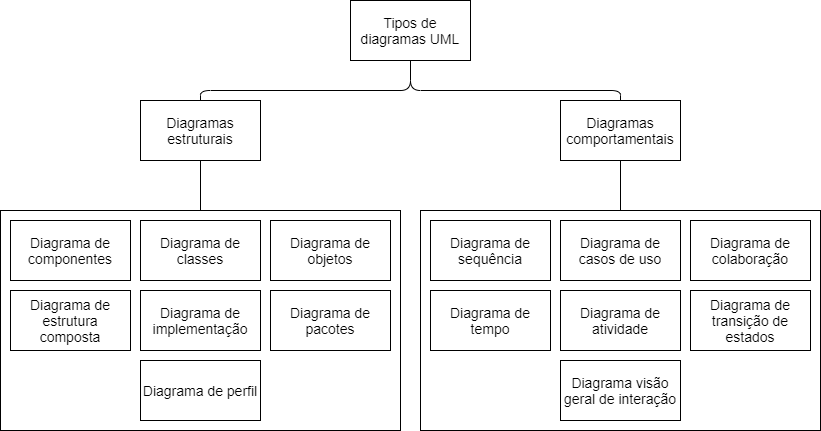
\includegraphics[scale=0.55]{uml-overview.png}
    \caption{Tipos de diagramas UML}
    \label{fig:umloverview}
\end{figure}

A partir dos tipos de diagramas disponíveis, foram utilizados apenas seis deles. Esses seis diagramas foram escolhidos a partir do objetivo que cada modelagem deveria atender. 

O primeiro deles tem a necessidade de modelar as funcionalidades necessárias para os atores que estão envolvidos com o sistema, representando os seus casos de uso. Por isso, esta diagramação foi feita utilizando o diagrama de casos de uso.

Para cada funcionalidade, foi necessário um diagrama que representasse a sequência de trocas de mensagens entre os objetos do sistema, e o diagrama UML utilizado que possui esse propósito é o diagrama de sequência.

Com o propósito de clarificar o que uma funcionalidade deve fazer, trazendo melhor documentação e explicação sobre a mesma, foi utilizado o diagrama de atividades. Esse diagrama é, essencialmente, um gráfico de fluxo que mostra o fluxo de controle entre uma atividade para outra. Neste trabalho, isso envolve a modelagem das etapas sequenciais de uma funcionalidade.

Como o sistema foi desenvolvido utilizando programação orientada a objetos, um diagrama para representar as classes, atributos, métodos e o relacionamento entre elas foi necessário. O diagrama que atende essa necessidade e foi utilizado no trabalho é o diagrama de classes.

Para representar a arquitetura de software do aplicativo móvel desenvolvido foi utilizado o diagrama de pacotes. Ele descreve os pacotes do sistema mostrando as dependências entre eles e o agrupamento de suas classes.

Por último, um diagrama que abrangesse o sistema como um todo, que represente o aplicativo cliente, o BD e outros componentes do sistema foi necessário. O diagrama de componentes tem exatamente esse propósito. Este diagrama mostra o relacionamento entre diferentes componentes de \textit{software} do sistema.

O principal objetivo e benefício da aplicação dessas modelagens é trazer eficiência no processo de desenvolvimento do sistema. Como toda análise foi feita anteriormente, essa eficiência é consequência da facilidade de visualização do sistema, documentação das decisões tomadas e ajuda a entender um sistema complexo dividindo-o em pequenas partes bem estruturadas.

\section{Arquitetura limpa}\label{sec:clean}

A arquitetura limpa, ou comumente conhecida como \textit{Clean Architecture}, foi criada por \textcite{cleanarchitecture} em seu livro \textit{Clean Architecture: A Craftsman’s Guide to Software Structure} e ela fornece uma metodologia de desenvolvimento que facilita o desenvolvimento de código, permite melhor atualização, manutenção e menos dependências entre os componentes do \textit{software}.

Um dos objetivos da arquitetura limpa é o princípio de \textit{design} de código conhecido como \Sigla{\textit{Separation of Concerns}}{SoC}. Esse objetivo é atingido a partir da separação do \textit{software} em camadas com diferentes responsabilidades.

Algumas das vantagens dessa separação por camadas são:

\begin{itemize}
    \item Testabilidade: As regras de negócio desenvolvidas no sistema poder ser testadas isoladamente, ou seja, sem  \Sigla{\textit{User Interfaces}}{UI}, bancos de dados ou agentes externos;
    \item Independente de UI: As interfaces podem ser modificadas frequentemente sem haver a necessidade de modificar o resto do \textit{software};
    \item Independente de BD: O sistema não está preso a nenhum tipo de BD específico e pode ser trocado sem afetar as regras de negócio;
    \item Independente de agentes externos: As regras de negócio não conhecem nada externo ao sistema;
\end{itemize}

\begin{figure}[!htb]
    \centering
    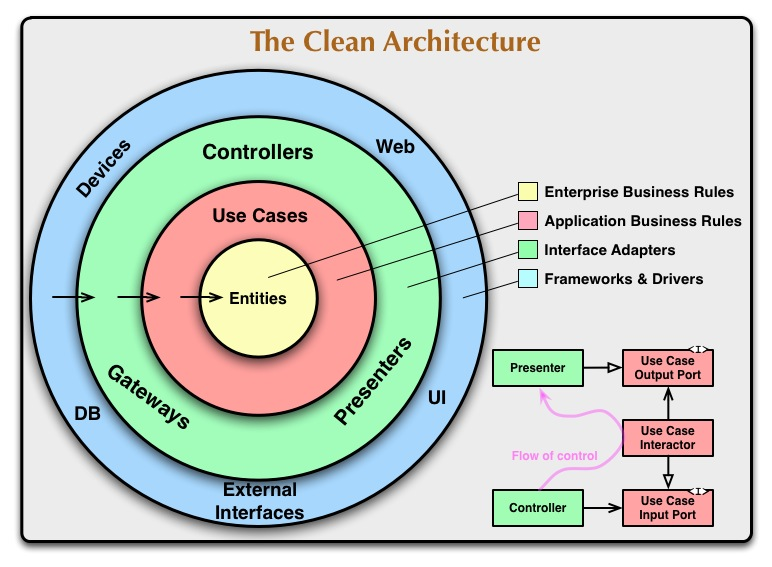
\includegraphics[scale=0.55]{CleanArchitecture.jpg}
    \caption[Arquitetura limpa]{Arquitetura limpa. Fonte: \cite{clean}}
    \label{fig:clean1}
\end{figure}

Cada círculo da \Figura{fig:clean1} representa diferentes áreas do sistema. Essas áreas só podem depender de outras mais internas, ou seja, a dependência só pode ocorrer "para dentro" do diagrama. A partir disso, nenhuma área conhece outras que sejam externas à ela. 

Essa regra de dependência, representada pelas setas da \Figura{fig:clean1},   garante que o sistema seja totalmente testável e poupa o desenvolvedor de problemas futuros com manutenções. Como o sistema é independente de camadas externas, como por exemplo \textit{frameworks} e bancos de dados, no momento que for necessário efetuar a mudança destes, o processo será mais simples e garantirá a integridade das regras de negócio.

Segundo \textcite{clean} e levando em consideração a legenda da \Figura{fig:clean1}, cada camada possui as seguintes definições:

\begin{itemize}
    \item \textit{Enterprise Business Rules}: são os objetos de domínio da aplicação que encapsulam as regras gerais e de alto nível. Eles aplicam lógicas gerais para toda a entidade;
    \item \textit{Application Business Rules}: são as ações do negócio, ou seja, contém as regras de negócio dos casos de uso do sistema. Esses casos de uso orquestram o fluxo de dados que são enviados e recebidos das entidades, direcionando-as para atingir um objetivo específico do caso de uso;
    \item \textit{Interface Adapters}: Essa camada é responsável por transformar as estruturas de dados dos casos de uso para o formato adequado aos agentes externos, como bancos de dados ou \textit{frameworks}, ou o contrário, convertendo os dados vindos dos agentes externos para a estrutura esperada pelos casos de uso;
    \item \textit{Frameworks \& Drivers}: Essa camada é composta por \textit{frameworks} ou ferramentas, como o BD. Nela é feita a ligação entre os agentes externos com a próxima camada mais interna ao círculo;
\end{itemize}

A arquitetura limpa não implica regras de apenas utilizar essas quatro camadas citadas anteriormente, isso significa que existem casos em que mais camadas podem ser utilizadas. Entretanto, a regra de dependência sempre deve ser aplicada mesmo nas novas camadas, e quanto mais interna ela for, mais abstrata ela deve se tornar.

A regra de dependência é clara, mas existem situações em que uma camada interna precisa chamar uma externa à ela. Por exemplo, o canto inferior direito da \Figura{fig:clean1} mostra os \textit{controllers} e \textit{presenters} se comunicando através da camada de caso de uso. Analisando o fluxo, ele começa no \textit{controller}, passa pelos casos de uso e termina no \textit{presenter}.

Essa violação da regra de dependência, onde o caso de uso invoca o \textit{presenter}, é resolvida através do princípio de inversão de dependências. Para isso, abstrações são utilizadas para que as dependências do código-fonte se oponham ao fluxo apenas nas fronteiras das camadas.

Considere o exemplo da necessidade do caso de uso chamar o \textit{presenter}. O caso de uso não deve chamar o \textit{presenter} diretamente, porque nesse caso ele violaria a regra de dependência. Então o caso de uso chama uma interface em sua camada, e as implementações dos métodos expostos pela interface são feitas pela camada \textit{presenter}.

Com isso, através do polimorfismo são criadas dependências no código que se opõem ao fluxo de controle para que o código esteja em conformidade com a regra de dependência, independente da direção que o fluxo de controle está indo.

Construindo a aplicação a partir dessas regras e princípios fazem com que o sistema seja testável, de fácil manutenção, já que a troca de \textit{frameworks} e bancos de dados podem ser realizadas sem impactar as camadas internas, criações de novas funcionalidades e refatorações podem ser feitas com mais facilidade e segurança, porque o código estará coberto de testes e a separação por camadas diminui o acoplamento, que minimiza o impacto de cada modificação.

\section{Padrão de Repositório}\label{sec:repositorypattern}

O padrão de repositório é um \textit{framework} conceitual responsável por encapsular um conjunto de objetos persistidos em um armazenamento de dados e as operações realizadas sobre eles, provendo uma visão orientada à objetos da camada de persistência da aplicação \cite{patterns}.

Segundo \textcite{ddd}, alguns dos benefícios da utilização desse padrão são:

\begin{itemize}
    \item Interface simples para obter e gerenciar o ciclo de vida de objetos persistidos;
    \item Desacopla a camada de domínio da aplicação da camada de persistência de dados;
    \item Permite fácil substituição da implementação, facilitanto o desenvolvimento de testes;
\end{itemize}

O repositório será utilizado para atender a regra de dependência da arquitetura limpa, fazendo com que os casos de uso não dependam da implementação das consultas feitas aos agentes externos, que estão presentes em camadas mais exteriores.

No processo de modelagem da arquitetura da aplicação, presente na Seção \ref{sec:modelagem}, é explicitado com detalhes a maneira que o padrão será utilizado no sistema.

\section{\textit{Frameworks} híbridos}\label{sec:flutter}
% Flutter 
Um dos principais requisitos do projeto é que o aplicativo deve funcionar em diversos tipos de sistemas operacionais de dispositivos móveis. Os dois principais do mercado são o \textit{Android} e o \textit{iOS}, que representam a grande maioria dos dispositivos.

Com isso, as linguagens de programação nativas de cada sistema foram excluídas, e os dois principais \textit{frameworks} híbridos utilizados no mercado são o \textit{Flutter} e o \textit{React}.

A decisão pela utilização do \textit{Flutter} aconteceu por alguns fatores. O principal deles foi o fato deste \textit{framework} ter sido lecionado durante uma disciplina cursada na graduação, outro fator foi em relação a existência de uma grande comunidade ativa e receptiva, que como consequência disso já produziu muitas documentações e tutoriais envolvendo a solução, e por último, a curva de aprendizado, que por conta da experiência prévia e da grande quantidade de materiais disponíveis na internet, se torna menor quando comparada ao \textit{React}.

\section{Princípios SOLID}\label{sec:solid}
% Principios SOLID
Os princípios SOLID serão utilizados no desenvolvimento do aplicativo por conta dos grandes benefícios que sua aplicação traz ao desenvolvimento de software e em relação a qualidade do código resultante dessa aplicação. SOLID é um acrônimo mnemônico dos 5 princípios de programação orientada a objetos introduzidos por \textcite{unclebob} em seu artigo \textit{Design Principles and Design Patterns}, onde cada letra representa um desses princípios.

Em seu artigo, Robert afirma que o software está em constante mudança e evolução, e conforme essa mudança acontece, a complexidade aumenta cada vez mais. Por conta disso, sem bons princípios de design de código, o software acaba se tornando de difícil manutenibilidade, testabilidade, legibilidade e extensibilidade. Os princípios SOLID foram desenvolvidos para combater esses problemas.

O objetivo geral desses princípios é reduzir as dependências para que diferentes áreas possam evoluir independentemente sem impactar umas às outras. Além disso, também possuem o propósito de construir designs fáceis de serem entendidos, mantidos, estendidos, escalados, reutilizados e testados. Por fim, a adoção dessas práticas evitam que problemas comuns no processo de desenvolvimento sejam enfrentados e possibilita a construção de software ágil, adaptável e eficiente.

Cada uma das letras do acrônimo representa um princípio, e são utilizados pela grande maioria dos sistemas desenvolvidos nos dias de hoje.

\subsection{Princípio da responsabilidade única}
A letra “S” do acrônimo representa o \textit{Single Responsibility Principle}, esse princípio tem relação direta com a coesão. Isso quer dizer que uma classe só terá uma única responsabilidade bem definida.

Em seu artigo, Robert descreve esse princípio dizendo que uma classe deve ter apenas um motivo para ser modificada; o que resulta na alta coesão citada no parágrafo anterior.

\subsection{Princípio aberto/fechado}
A letra “O” representa o \textit{Open/Closed Principle}, esse princípio foi descrito por Robert da seguinte forma: 

\begin{quotation}
"Devemos escrever nossos módulos de forma que possam ser estendidos, sem exigir que sejam modificados. Em outras palavras, queremos ser capazes de mudar o que os módulos fazem, sem alterar o código-fonte dos módulos."
\end{quotation}

Ou seja, Robert está se referindo ao conceito abstrato da extensão. Usar heranças ou interfaces que permitem polimorfismo é uma das maneiras mais comuns de cumprir esse princípio.

\subsection{Princípio substituição de Liskov}
A letra “L” do acrônimo significa \textit{Liskov Substitution Principle}, esse princípio prega que uma classe derivada deve ser substituível por sua classe base; essa frase é a simplificação da definição científica que foi apresentada por \textcite{liskov} no artigo \textit{Behavioral Subtyping Using Invariants and Constraints}.

A definição traduzida apresentada no artigo científico é:

\begin{quotation}
“Se $\theta(x)$ é uma propriedade provável dos objetos $x$ do tipo $T$. Então $\theta(y)$ deve ser verdadeiro para objetos $y$ do tipo $S$ onde $S$ é um subtipo de $T$.”
\end{quotation}

\subsection{Princípio segregação de interfaces}
A letra "I" representa o princípio \textit{Interface Segregation Principle}, em que Robert diz que muitas interfaces específicas para o cliente são melhores do que uma grande interface de propósito genérico.

Para os desenvolvedores, isso significa que novos métodos ou funcionalidades não devem ser criados a partir de uma interface existente, ao invés disso, é recomendado que se crie uma nova interface e as classes poderão implementar múltiplas interfaces conforme for necessário.

\subsection{Princípio da inversão de dependências}\label{sec:D}
A última letra do acrônimo, a letra "D", representa o princípio \textit{Dependency Inversion Principle}, ele oferece uma maneira de desacoplar módulos do \textit{software}.

Robert explica esse princípio dizendo que módulos de alto nível não devem depender dos de baixo nível, ambos devem depender de abstrações. Além disso, as abstrações não devem depender dos detalhes, os detalhes que devem depender das abstrações.

\section{Arquitetura orientada a eventos}\label{sec:eventos}
% Arquitetura orientada a eventos
Segundo a \textcite{redhat}, a arquitetura orientada a eventos é um modelo de \textit{design} de sistemas que não depende de linguagens de programação ou \textit{frameworks}, porque nele é abordado como modelar seu sistema de maneira agnóstica à linguagens.

Aplicando essa arquitetura, o acoplamento entre serviços no sistema é mínimo, ou seja, os diferentes componentes do sistema não terão altas dependências diretas entre si. Isso acontece porque os produtores dos eventos não conhecem os consumidores e o evento em si não conhece as consequências de sua ocorrência. Portanto, o principal benefício trazido pela arquitetura é que o sistema se torna flexível, se adapta a mudanças e toma decisões em tempo real.

A definição de um evento é uma mudança de estado no \textit{software} ou \textit{hardware}. Quando essa mudança acontece, uma mensagem é enviada por uma parte do sistema para avisar outra parte que alguma mudança ocorreu.

Com base nas definições apresentadas, a arquitetura orientada a eventos é composta por produtores e consumidores de eventos. O papel do produtor é detectar eventos e os representar como uma mensagem, que é enviada por meio de canais, que serão posteriormente processadas de maneira assíncrona pelo consumidor. O consumidor detectará novas mensagens publicadas no canal de comunicação e processará esse evento a partir das informações contidas nele. 

Existem diferentes tipos de arquitetura orientada a eventos, o modelo utilizado neste trabalho será o \textit{pub/sub}. \textit{Pub/sub} é o nome utilizado para representar o modelo \textit{Publish/Subscribe}, trata-se de uma infraestrutura de mensageria baseada em subscrições em um fluxo de eventos, ou seja, após ocorrer um evento, ele será publicado em um sistema de mensagens assíncronas, em que haverá um consumidor que receberá a publicação.

A maneira que o sistema desenvolvido neste trabalho utiliza o modelo \textit{pub/sub} é explicado no Capítulo \ref{chp:desenvolvimento}.

\section{Banco de dados orientado a documentos}\label{sec:bd}
% Banco de dados orientado a documentos
O banco de dados orientado a documentos é um tipo de BD não-relacional que armazena e consulta dados em formato \Sigla{JavaScript Object Notation}{JSON}, cuja principal característica é a organização de dados livres de esquemas. Por conta disso, esse tipo de banco facilita as consultas feitas pelos desenvolvedores, que usam o mesmo formato de modelo que usam no código do aplicativo.

Outras características desse tipo de BD \textit{NoSQL} é a sua natureza semiestruturada, flexível e hierárquica dos documentos, que permite que o banco evolua conforme as necessidades do aplicativo.

\section{Fluxo de trabalho com \textit{Git}}\label{sec:Git}
% Fluxo de trabalho com Git
Este projeto foi desenvolvido utilizando um sistema de controle de versão chamado \textit{Git}. Ele foi escolhido por ser a ferramenta mais utilizada pela comunidade de desenvolvimento de \textit{software}, gratuita e de código aberto. A utilização de um sistema de versionamento foi por conta dos benefícios citados abaixo.

\begin{itemize}
    \item Registra todo o histórico de alterações dos arquivos. Isso significa que serão salvas todas as alterações de conteúdo, deleção ou adição dos arquivos, o autor, data e mensagens escritas em cada alteração.
    \item Facilidade na reversão de alterações, ou seja, caso uma nova funcionalidade não se comporte da maneira esperada e cause falhas no aplicativo, a reversão para alguma versão anterior é feita a partir do histórico registrado pelo versionamento.
    \item Suporte a ramificações e mesclas, que possibilitam a criação de diferentes linhas de desenvolvimento independente uma das outras, e posteriormente da mesclagem dessas linhas em uma ramificação principal, que conterá todo código testado e validado do projeto.
\end{itemize}

Apesar do \textit{Git} ser uma ferramenta robusta para o desenvolvimento, existem alguns tipos de fluxos de trabalhos que são adotados para desenvolver um projeto. Os fluxos de trabalho procuram padronizar a maneira que os desenvolvedores colaboram dentro do projeto, a nomeação de ramificações, a responsabilidade que cada tipo possui e a maneira que novas funcionalidades são integradas ao código principal.

Por conta de sua robustez, padronização e organização elevada, o fluxo de trabalho utilizado neste projeto foi o \textit{GitFlow}, criado por \textcite{gitflow}. Ele é ideal para gerenciar projetos grandes, com ciclo de lançamento agendado e atribui responsabilidades específicas para cada tipo de ramificação.

Existem 5 tipos de ramificações nesse fluxo de trabalho, sendo elas a \textit{main}, \textit{develop}, \textit{hotfix}, \textit{release} e \textit{feature}.

A \textit{main} e a \textit{develop} armazenam todo o histórico de alterações do desenvolvimento de um produto. Cada modificação na ramificação \textit{main} representa uma nova versão lançada para os usuários, e a ramificação \textit{develop} contém as iterações das funcionalidades que são desenvolvidas. Portanto, uma modificação na ramificação \textit{main} representa um conjunto de funcionalidades que foram iteradas na ramificação \textit{develop}.

A \Figura{fig:gitflow1} representa a evolução independente das duas ramificações, para melhor visualização desse diagrama e dos próximos, cada ramificação é representada por uma cor e a primeira letra de seu nome. 

\begin{figure}[!htb]
    \centering
    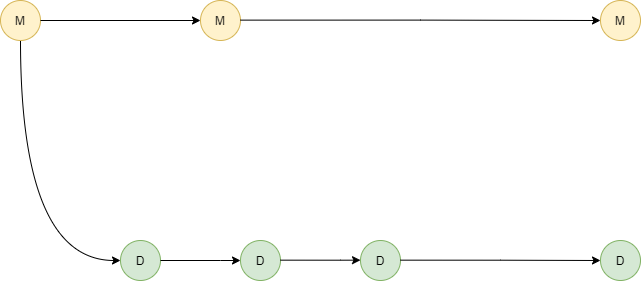
\includegraphics[scale=0.65]{gitflow-master-develop.png}
    \caption{Representação das ramificações \textit{main} e \textit{develop}}
    \label{fig:gitflow1}
\end{figure}

Para o desenvolvimento de novas funcionalidades é utilizada a ramificação \textit{feature}. Ela deve ser derivada da \textit{develop} e mesclada logo após a finalização do desenvolvimento da funcionalidade, como mostra a \Figura{fig:gitflow2}.

\begin{figure}[!htb]
    \centering
    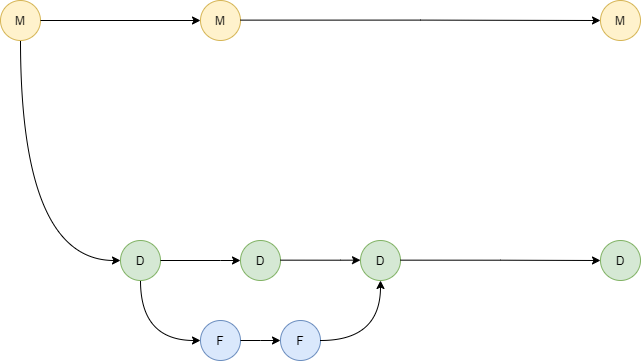
\includegraphics[scale=0.65]{gitflow-feature.png}
    \caption{Representação das ramificações \textit{main}, \textit{develop} e \textit{feature}}
    \label{fig:gitflow2}
\end{figure}

Depois de algumas iterações de funcionalidades na \textit{develop}, é criado uma preparação para um lançamento de uma nova versão do produto. Essa preparação é feita pela ramificação \textit{release}. Nela, nenhuma funcionalidade é desenvolvida, apenas pequenos ajustes em possíveis falhas ou documentações, como mostra a \Figura{fig:gitflow3}.

É importante ressaltar que a \textit{release} é derivada da \textit{develop} e deve ser mesclada com a \textit{main} e com a  \textit{develop} novamente, já que algumas atualizações no código podem ter sido feitas na ramificação \textit{release}. Quando a mesclagem para a \textit{main} for feita, uma nova versão do produto é lançada.

\begin{figure}[!htb]
    \centering
    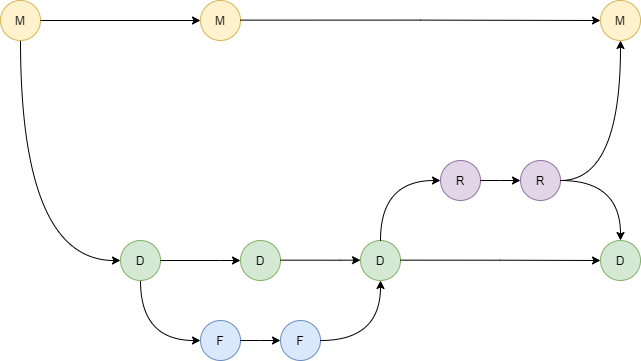
\includegraphics[scale=0.65]{gitflow-release.png}
    \caption{Representação das ramificações \textit{main}, \textit{develop}, \textit{feature} e \textit{release}}
    \label{fig:gitflow3}
\end{figure}

A última ramificação que esse fluxo de trabalho possui é a \textit{hotfix}. Ela é responsável por fazer pequenas alterações diretamente na main, ou seja, eventuais falhas que foram entregues aos usuários são corrigidas nesta ramificação.

A  \Figura{fig:gitflow4} mostra a \textit{hotfix} atualizando alguma falha que estava na \textit{main} e como todas as 5 ramificações estão presentes, consequentemente representa um ciclo completo utilizando o \textit{GitFlow}.

\begin{figure}[!htb]
    \centering
    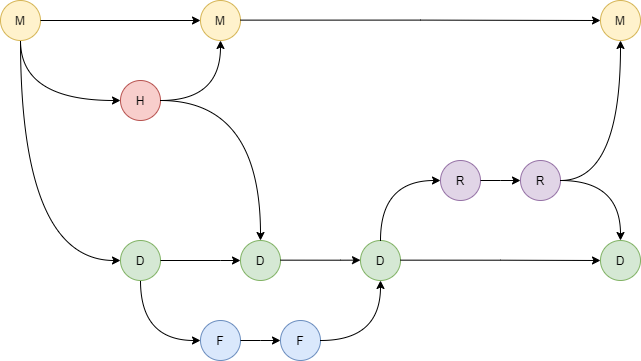
\includegraphics[scale=0.65]{gitflow-final.png}
    \caption{Representação de todas ramificações do \textit{GitFlow}}
    \label{fig:gitflow4}
\end{figure}


\section{\textit{Pipelines} de integração e entrega contínua}\label{sec:pipelines}
% Pipelines de CI/CD
Como já citado anteriormente, a qualidade do software é uma preocupação importante no processo de desenvolvimento deste projeto. Aliado a isso, a criação de pipelines trás benefícios ao sistema, alguns deles são:
\begin{itemize}
    \item Maior taxa de entrega: em conjunto com o fluxo de trabalho adotado no desenvolvimento, a frequência com que novas funcionalidades ou correções de falhas são lançadas é maior. Como o processo de entrega é automatizado, o desenvolvedor foca no desenvolvimento de novas entregas, e não em passos repetitivos para efetuá-las;
    \item Confiabilidade de testes: os testes são efetuados de forma automática, e caso algum teste falhe, a entrega é impossibilitada de ser feita, garantindo que apenas pedaços de código validados possam ser entregues aos clientes;
    \item Redução de custos: menos tempo gasto em processos manuais e repetitivos, e mais tempo desenvolvendo novas funcionalidades resulta em redução de custos, já que o desenvolvedor se preocupa somente com atividades que agregam valor;
\end{itemize}

Os \textit{pipelines} de \Sigla{\textit{Continuous Integration and Continuous Delivery}}{CI/CD} são um conjunto de etapas que integram com o código principal, efetuando principalmente testes nesse novo código, e o entregam, que seriam novas versões liberadas aos clientes.

Existem diversas ferramentas de CI/CD, e a ferramenta escolhida foi o \textit{GitHub Actions}, porque possui integração perfeita com a central de repositórios \textit{git} que será utilizada, o \textit{GitHub}. Além disso, a ferramenta é gratuita, suporta as principais funcionalidades que um \textit{pipeline} precisa e possui boa documentação.

\section{\textit{Serviços computacionais na nuvem}}\label{sec:googlefirebase}
% Firebase
Durante o processo de desenvolvimento, surgiu a necessidade do sistema possuir serviços remotos na nuvem, tais como BD e um servidor \textit{backend}, onde rotinas pudessem rodar independentemente do dispositivo móvel do usuário.

Essa necessidade trouxe o requisito de se utilizar serviços computacionais na nuvem. Levando em consideração as tecnologias e os requisitos do aplicativo, o provedor utilizado foi o \textit{Firebase}.

Esse provedor de nuvem é especializado em acelerar o processo de desenvolvimento de sistemas \textit{mobile}, fornecendo ferramentas de fácil configuração, auto gerenciadas e de alta qualidade.

Os serviços que foram utilizados do provedor foi o BD orientado a documentos, o servidor \textit{backend} para executar as rotinas de rastreamento de contatos e um sistema de mensageria responsável por enviar ao \textit{backend} os eventos de escrita ocorridos em coleções específicas no BD.

Além da alta disponibilidade e confiabilidade dos serviços oferecidos pelo \textit{Firebase}, esse conjunto de tecnologias é uma escolha comum para aplicações móveis que utilizam \textit{Flutter}. A comunidade de desenvolvimento possui diversos tutoriais e documentações que abrangem os mais diversos casos de uso que podem ser utilizados em conjunto, o que facilitou o processo de desenvolvimento.

Cada um dos recursos oferecidos pela plataforma são explicados no Capítulo \ref{chp:infraestrutura}, e a forma de como foram utilizados está descrita no Capítulo \ref{chp:desenvolvimento}.